\section{問題とその背景}\label{sec:introduction}

縦横比$\lambda=3$において、数値探索は参照座標で$0.823938$付近に停留半径を見出す。その点を回転させると円が得られる。第二の半径、あるいは赤道面の外の停留点を排除するものは何か。正規化した動径方向微分$H$の探索的な三次元被覆では、31,340個の終端の箱のうち21,254個で符号が分離されないまま残った。これらの箱は、停留点を数えるものでも、分類定理の破綻を数えるものでもない。これらは、第一の実験が答えられなかった問いがどれであるかを正確に教えてくれる。

第二の実験は、赤道から離れたところで鉛直方向微分を用い、次いで赤道上でスカラーの交差を数えた。本稿で報告する第三の実験は、点での値が示唆するより強い赤道上の単調性が、領域全体の包囲のもとでも成り立つかを問う。第一の実験は中実の子午線領域と形状区間を被覆し、第三の実験は赤道半径と形状のみを被覆する。各実験はそれぞれ自身の領域の上で用いる。これらを合わせると、族全体に対する問いが動機づけられる：停留成分の個数、次元、型は形状とともにどのように変化するか。

極値を与える中心はこの問いの一部である。鞍点も重要である。鞍点は、極値を選ぶ選択規則では捨てられてしまう停留構造の変化を記録するからである。回転楕円体はとりわけ扱いやすい試験例を与える：球の停留点は一つであるが、回転対称性は、中心から離れたところに、孤立した軸上の臨界点の対と円状の臨界多様体の両方を許す。本分類の目的は、これらの集合がいつ現れるかを決定し、非コンパクトな形状区間にわたって追加の成分を排除することである。

% Internal, AI-assisted research draft.  Author verification and the target
% journal's current AI policy must be resolved before submission.
% Bibliography keys are defined in ../references_additions.bib.
\subsection{関連する中心の問題と動機}
\label{subsec:related-centers}

物体の内部に特別な点を選ぶことには、変分的な観点からの相当な
歴史がある。Moszy\'nskaの動径中心は、選んだ点からの動径距離の関数の球面
平均を最大化することで定義され、
凸体に対しては、凹かつ狭義単調増加な平均化プロファイルが一意的な
最大点を与える\citep{moszynska2000selectors}。O'Haraは、Rieszポテンシャルと
その正則化から一般化された中心を展開している
\citep{ohara2012renormalization}。ポテンシャルの次数を$\beta$と書くと、
正則化していない式は次のとおりである：
\[
 V_{\Omega}^{(\beta)}(p)
   =\int_{\Omega}|x-p|^{\beta-n}\,dx,\qquad \beta>0.
\]
問題となる極値は次数に依存し、$\beta=n$では対数による置き換えが、
非正の次数では正則化が伴う。滑らかな凸体
$K\subset\mathbb R^3$と$0<\beta<3$に対して、このRieszポテンシャルの発散定理による
表示は次のとおりである：
\[
 V_{K}^{(\beta)}(p)
  =\frac{1}{\beta}\int_{\partial K}|x-p|^{\beta-3}
       (x-p)\cdot n(x)\,dA(x).
\]
幾何学的な因子$(x-p)\cdot n(x)\,dA(x)$は、まさに
以下で用いる基点に依存する錐体積の重みである。O'Haraのポテンシャルは
これに距離のべきを掛けて、極値を与える
中心を選ぶのに対し、本論文のエネルギーはこれに、動径方向と外向き法線の間の
角の二乗を掛け、
回転楕円体の軸比が変わるときのすべての停留成分を調べる。これらの構成は、
基点そのものを幾何学的汎関数の変数として
扱うことの自然な先例を与える。

これらの文献における一意性は、汎関数と物体の幾何の
両方に依存する。O'Haraは、与えられた各ポテンシャル次数において、非球面性が十分小さいとき、極値を与えるRieszポテンシャル中心の
一意性を証明している\citep{ohara2022nearly}。Sakataは、
狭義単調減少な動径核をもつポテンシャルの最大点を研究し、
一意性のための追加の十分条件を証明し、
最大点が二つ以上ある例を調べている\citep{sakata2016uniqueness}。とくに、平面の円環
$A=\{y\in\mathbb R^2:1\leq|y|\leq2\}$に対しては、その
$r^{-1/2}$ポテンシャル中心の集合は円であり、円板の和集合は
そのような中心を二つもちうる。これらの例は非凸な平面領域であるが、
本論文の円はこれに対し、凸な三次元の扁長
回転楕円体の内部における角度エネルギーのMorse--Bott\emph{鞍点}集合として
現れる。これらの例は、極値集合の構造に
注意深く目を向ける動機となるが、ここで考える角度
汎関数の停留集合を分類するものではない。また、選ばれた大域的
極値点の一意性は、それだけでは、別の
汎関数のすべての臨界点を記述するものでもない。

我々の問題は、$p$から境界点$x$へ向かう方向と
$x$における外向き法線との間の角の二乗を、次の
基点に依存する確率測度で平均したものに関わる：
\[
 d\mu_{K,p}(x)
   =\frac{(x-p)\cdot n(x)}{3\,\operatorname{Vol}(K)}\,dA(x)
   \qquad (p\in\operatorname{int}K).
\]
したがって、この定義には、視線
方向と重みに加えて法線場も関わる。我々は、このエネルギーを動径核の
体積ポテンシャルと同一視せず、これに対して前述の一意性定理を援用することもしない。
その代わりに、$p$に関する導関数が
消える集合の全体を調べる。回転楕円体族については、パラメータ$\lambda$は体積を固定して形状を
変えるものであり、Riesz核の次数$\beta$ではない。目的は、
中心の臨界点、軸上の対、および回転対称な
臨界円が、それらの退化と境界への接近も含めて、
一つの停留集合の図式にどのように収まるかを決定することである。

動径Gauss写像は、凸体の境界上で、動径方向に外向き
法線を対応させる。Gauss像
問題におけるその役割は、B\"or\"oczky, Lutwak, Yang, Zhang, Zhaoによって研究されている
\citep{boroczky2020gaussimage}。我々の汎関数にも、これと同じ
動径–法線の対応が現れるが、基点$p$は物体の内部を
動く。比較のために述べると、BertrandによるGauss曲率
指定問題の最適輸送による定式化では、（同論文の式~(6)において）外向き法線
$n$と動径方向$u$の間の角度コスト
$c(n,u)=-\log\cos d_{\mathbb S^2}(n,u)$が用いられる\citep{bertrand2016gauss}。ここでは
コストはその代わりに角の二乗$d_{\mathbb S^2}(n,u)^2$であり、これを
錐体積の確率測度に関して平均するが、その停留点を分類するためにGauss像の定理や
曲率指定の定理を援用することはしない。

熱流の中心は、関連するが別種の比較対象を与える。
MagnaniniとSakaguchiは、温度が
$u_t=\Delta u$を満たし、初期温度が$1$、境界温度が$0$である有界な伝導体を研究している
\citep{magnaniniSakaguchi2004hotspot}。ホットスポットとは$u(\,\cdot\,,t)$を最大にする点であり、
彼らの定常ホットスポットの問題は、同じ点がすべての正の時刻において
最大点であり続けるかどうかを問う。そこで述べられている凸な伝導体の問題では、
固定した各正の時刻において、空間的な臨界点はただ一つである。
ここで調べる条件は、固定した各形状における$d_p E_\lambda=0$であり、
極値点だけでなく鞍点も含む。その定義に
熱の時間発展は現れない。したがって、角度の
問題に鞍点円が現れることは、ホットスポットの一意性の結果から導かれることも、それと矛盾することもない。

非有界な形状の範囲にわたってそのような図式を確立するには、
解析的な簡約と数値的な検証とを結ぶものが必要である。この結びつきは、
計算機援用証明の確立された実践に属するものであり、
Tuckerによる常微分方程式の厳密な解析がその例であって、彼による精度保証付き
数値計算の解説およびG\'omez-Serranoの概説において説明されている
\citep{tucker2002rigorous,tucker2011validated,gomezSerrano2019survey}。
JohanssonのArbは、任意精度の
中心半径型演算の標準的な実装を提供し\citep{johansson2017arb}、彼の後の
論文は、ボール演算における厳密な数値積分を記述している
\citep{johansson2018integration}。演算による包囲
だけでは、特定の積分核の正しさや
領域被覆の完全性は確立されない。証明は、どの
不等式が排除、存在、一意性、および型を導くのか、また
有限被覆が解析的な端点領域とどのように接続するのかも、明示しなければならない。我々は、
精度保証付き数値計算の枠内での、公式、
包囲、および検査のこの問題固有の組織化を\emph{GeoEnclosure}と呼ぶ。


区間Newton判定とKrawczyk判定は、箱の内部の正則な根を分離できる\citep{intervalNewton}。分枝刈り込み型の解法は、局所的な判定と孤立根の大域的な探索とを組み合わせる\citep{branchPrune}。半径多項式法は、Newton型写像が縮小写像となる球を見つけることで、局所一意性を証明できる\citep{radiiContinuation}。停留円においては、全勾配のJacobianが軌道に沿って至るところ特異であり、軌道のどの点も孤立していない。回転によって軌道座標が取り除かれ、スカラーの分離が意味をもつようになる。ここでの問題固有の寄与は、デカルト座標での接方向の四階導関数から動径方向の交差を復元すること、および直接の微分が接触に出会うところで弦Hessianの差に切り替えることである。被覆と分離の原理そのものは標準的である。

\paragraph{このエネルギーに関する先行研究。}
著者による以前の球に関する原稿は、球に対する同じ
停留点・最小点の結果を与えているが\citep{furutaSphere}、本論文の
命題~\ref{prop:sphere}の証明は自己完結しており、
その原稿に依拠しない。Furutaによる以前の扁長側の局所
分岐の計算\citep{furutaProlate}は、中心における赤道方向の二次係数の零点を、Arbによる端点評価によって
$[4.72438340452113340672,4.72438340452113340673]$の中に
分離している。その軸比は本論文の$\lambda$である。横断方向の長さの単位を変えても、二次係数に正の正規化定数を掛けても、この零点は変わらない。したがって、局所的な閾値と円の発生は本論文に先行する。大域的な議論にどの端点計算が入るのかを特定するために、表~\ref{tab:critical}には、我々の窓全体の被覆から得られるより広い挟み込み区間を残してある。同じプロジェクトの三軸の記録は、局所的な開折、Hessianの退化曲線の交わり、および二つの軸上のMorse指数を扱っている。明示的に述べた有限個の入力C1--C6のもとで、ここでの寄与は、それらの局所的な分岐を、軸比の全域にわたる停留集合の分類（軸上の鞍点対と赤道上のMorse--Bott鞍点円の範囲、それらが境界に到達する軸比、およびそれ以外の停留成分の排除）へと拡張することである\citep{furutaProlate,furutaTriax}。


証明は三つの段階からなる。第一に、解析的な公式によって、その符号が軸外または赤道外の停留点を排除するスカラー微分を特定する。第二に、一変数の議論によって、残る零点の個数と型を決定する。第三に、有限個の区間被覆と、退化する二つの端における明示的な評価が、これらの議論で用いる符号を与える。ここで\emph{basepoint geometry}という名称は第一の定式化を指し、\emph{GeoEnclosure}は、得られた式に対する確立された包囲法のこの適用を指す\citep{furutaGeoEnclosure2026}。いずれの名称も、区間演算、錐体積測度、臨界多様体が本研究に由来すると主張するものではない。

\section{エネルギー、座標、境界の規約}\label{sec:definition}

\subsection{動く基点のエネルギー}
$K\subset\R^3$を滑らかな狭義凸体とし、$p$を内点とし、$n(x)$で$x\in\partial K$における外向き単位法線を表す。次のように定める。
\begin{align}
 u_p(x)&=\frac{x-p}{|x-p|},&
 \alpha_p(x)&=\arccos\bigl(u_p(x)\cdot n(x)\bigr),\label{eq:angle}\\
 d\mu_{K,p}(x)&=\frac{(x-p)\cdot n(x)}{3\vol(K)}\,dA(x),&
 E_K(p)&=\int_{\partial K}\alpha_p(x)^2\,d\mu_{K,p}(x).\label{eq:energy}
\end{align}
角はラジアンで測る。狭義に内部にあることから$(x-p)\cdot n(x)>0$が従い、発散定理により次を得る。
\[
 \int_{\partial K}(x-p)\cdot n(x)\,dA(x)=3\vol(K).
\]
したがって$\mu_{K,p}$は確率測度である。角と重みはいずれも$p$に依存し、ともに微分しなければならない。この境界測度を法線写像で押し出すと、体積で正規化した$K-p$の錐体積測度が得られる\citep{Boroczky2013,Huang2016}。

このエネルギーは、平行移動、座標の直交変換、正の相似変換のもとで不変である。倍率$a$に対して、式~\eqref{eq:energy}の分子、面積要素、体積はそれぞれ$a,a^2,a^3$倍になる。一般のアフィン写像は角を変えるので、この汎関数を不変にするものではない。

被積分関数には幾何学的な解釈がある。境界を$x=p+r_p(u)u$、$u\in S^2$と書く。その外向き法線は$u-\nabla_{S^2}\log r_p$に平行である。動径射影によって、あるいは向き付けられた面積要素と$u$とのスカラー積をとることによって、$(x-p)\cdot n\,dA=r_p^3\,d\omega$を得る。よって次が成り立つ。
\[
 \tan\alpha_p=|\nabla_{S^2}\log r_p|,\qquad
 E_K(p)=\frac{1}{3\vol K}\int_{S^2}r_p^3
 \arctan^2\!\bigl(|\nabla_{S^2}\log r_p|\bigr)\,d\omega .
\]
この角は、対数動径距離の方向による変動を測る。エネルギーが消えるのは、動径距離が一定であるとき、すなわち$K$が$p$を中心とする球体であるとき、かつそのときに限る。

\subsection{体積保存回転楕円体}
次のように書く。
\begin{equation}\label{eq:family}
 K_\lambda=M_\lambda\B,\qquad
 M_\lambda=\diag(\lambda^{-1/3},\lambda^{-1/3},\lambda^{2/3}),\qquad\lambda>0.
\end{equation}
ここで$\B$は閉単位球体であり、基点を指定するときは常にその内部を考えるものとする。行列式は1であり、$\vol(K_\lambda)=4\pi/3$である。形状は$\lambda<1$のとき扁平、$\lambda=1$のとき球、$\lambda>1$のとき扁長である。$\lambda=0$も$\lambda=\infty$も族の元としては含めない。

$p=M_\lambda q$、$|q|<1$とおき、$\E_\lambda(q)=E_{K_\lambda}(M_\lambda q)$とおく。相似不変性により$L_\lambda=\diag(1,1,\lambda)$を用いることができる。$\xi\in\Sph$に対して次のようにおく。
\begin{align}
 k&=1-q\cdot\xi,& D&=|L_\lambda(\xi-q)|,& S&=|L_\lambda^{-\mathsf T}\xi|,\label{eq:reference_variables}\\
 \gamma&=\frac{k}{DS},& f(c)&=\arccos^2c,&
 \av{h}&=\frac1{4\pi}\int_{\Sph}h(\xi)\,d\Omega.\nonumber
\end{align}
このとき次が成り立つ。
\begin{equation}\label{eq:reference_energy}
 \E_\lambda(q)=\av{kf(\gamma)}.
\end{equation}
実際、$x=M\xi$に対して、曲面のJacobianは$\det M\,|M^{-\mathsf T}\xi|$であり、法線は$M^{-\mathsf T}\xi/|M^{-\mathsf T}\xi|$である。このJacobianに$(x-p)\cdot n=k/|M^{-\mathsf T}\xi|$を掛け、$3\vol(M\B)=4\pi\det M$を用いれば、式~\eqref{eq:reference_energy}が示される。

$\lambda$を固定すると、連鎖律により次を得る。
\begin{equation}\label{eq:coordinate_hessian}
 \nabla_q\E_\lambda=M_\lambda^{\mathsf T}\nabla_pE_{K_\lambda},\qquad
 \nabla_q^2\E_\lambda=M_\lambda^{\mathsf T}(\nabla_p^2E_{K_\lambda})M_\lambda.
\end{equation}
零点とHessianの慣性は保たれる。本原稿を通じて、微分の数値的な評価は参照変数$q$を用いる。その大きさをそのまま物理座標に写してはならない。

第三軸のまわりの回転と赤道に関する鏡映により、エネルギーは$\rho\ge0$として$\mathcal E_\lambda(\rho,z)=\E_\lambda(\rho,0,z)$に帰着する。これは$z$について偶である。中心はすべての$\lambda>0$に対して停留点である。内部のコンパクト部分集合上では、$D$は零から離れて有界である。$f$の導関数の$c=1$における見かけの特異性は除去可能であるから、以下で用いる内部での微分は正当である。

\subsection{有界な一階微分の核}
連続に拡張した関数を次のように定める。
\begin{align}
 P(c)&=-f'(c)=\frac{2\arccos c}{\sqrt{1-c^2}},& Q(c)&=2P(c)+cP'(c),\label{eq:PQ}\\
 J(c)&=cP(c)-f(c),& K(c)&=c^2P(c).\nonumber
\end{align}
$0\le c\le1$に対して次が成り立つ。
\begin{equation}\label{eq:PQbounds}
 P(c)=2\int_0^\infty\frac{dt}{\cosh t+c},\quad
 2\le P\le\pi,\quad -2\le P'\le0,\quad Q\ge\frac{10}{3}.
\end{equation}
最初の恒等式は$s=\tanh(t/2)$によって従う。その積分記号下での微分により、$P'$に対する評価と次の式が得られる。
\[
 Q(c)=2\int_0^\infty\frac{2\cosh t+c}{(\cosh t+c)^2}\,dt.
\]
被積分関数は$c$について減少し、一方$P(1)=2$、$P'(1)=-2/3$、$Q(1)=10/3$である。

$u=L_\lambda(\xi-q)/D$とおき、$k_i=-\xi_i$と$D_i=-(L_\lambda)_{ii}u_i$を用いて式~\eqref{eq:reference_energy}を微分すると、次を得る。
\begin{equation}\label{eq:gradient}
 \partial_{q_i}\E_\lambda
 =\av{\xi_iJ(\gamma)-(L_\lambda)_{ii}S u_iK(\gamma)}.
\end{equation}
有限な$\lambda>0$を固定するごとに、この核は内部の$q$について一様に有界である。境界への極限$q\to q_0\in\Sph$において、核は唯一の接触点$\xi=q_0$（球面測度零の集合）を除いて各点収束する。優収束定理により、全勾配の一意な連続トレース$g_\partial(q_0;\lambda)$が得られる。この優関数による評価は、$\lambda$が$(0,\infty)$のコンパクト部分集合を動くときにも一様である。

\begin{definition}[境界零点の規約]\label{def:boundary}
境界零点集合は次で与えられる。
\begin{equation}\label{eq:boundary}
 Z_\partial(\lambda)=\{q\in\Sph:g_\partial(q;\lambda)=0\}.
\end{equation}
これは全勾配のトレースの零点集合であって、球面上の制約付き停留条件$(I-qq^{\mathsf T})g_\partial=0$ではない。
\end{definition}

用いるのは一階微分のトレースのみである。特に、境界Hessianの連続拡張は一切仮定しない。一般の境界点において軸方向成分の符号が定まれば、勾配成分が非零であることが確立される。それだけでは外向き法線方向微分の符号は決まらない。

\section{分類とその明示的な入力}\label{sec:classification}

$h_c(\lambda)=\partial_{q_1q_1}\E_\lambda(0)$および$a_c(\lambda)=\partial_{q_3q_3}\E_\lambda(0)$とおく。四つの臨界値を次のように表す。
\[
 0<\cO<\bO<1<\bP<\cP<\infty.
\]
これらは表~\ref{tab:critical}の零点と有理区間によって定められる。この表は、各定義関数に対して端点での符号を用いている。扁長側の中心に対する以前の局所的な包囲は、以下で比較する。最終列の小数近似は位置を示すものである。

\begin{table}[htbp]\centering\small
\caption{臨界パラメータ。$(a,b)/2^m$は$(a/2^m,b/2^m)$を意味する。小数値は位置を示すのみである。}\label{tab:critical}
\begin{tabular}{@{}llll@{}}\toprule
値 & 定義する零点 & 記録された有理区間 & 参考小数値\\\midrule
$\cO$ & $a_c$ & $(407958860300,407958860301)/10^{12}$ & $0.40795886030$\\
$\bO$ & 極での軸方向トレース & $(674802,674811)/2^{20}$ & $0.64354577$\\
$\bP$ & 赤道での動径方向トレース & $(34651360,34651369)/2^{24}$ & $2.06538229$\\
$\cP$ & $h_c$ & $(79261996,79262005)/2^{24}$ & $4.72438340$\\\bottomrule
\end{tabular}
\end{table}

$O=\{0\}$と書き、存在するときには次のようにおく。
\begin{align}
 A_\lambda&=\{(0,0,z_*(\lambda)),(0,0,-z_*(\lambda))\},\quad 0<z_*<1,\label{eq:axial_set}\\
 C_\lambda&=\{(\rho_*(\lambda)\cos\phi,\rho_*(\lambda)\sin\phi,0):0\le\phi<2\pi\},\quad 0<\rho_*<1.\label{eq:circle_set}
\end{align}
$P_\pm=\{(0,0,1),(0,0,-1)\}$とし、$C_\partial$を単位赤道円とする。物理的な集合は$M_\lambda$を施して得られる。

\begin{theorem}[計算主張C1--C6からの分類]\label{thm:classification}
第~\ref{sec:computational}節に明示的に述べる計算主張C1--C6を仮定する。エネルギー~\eqref{eq:reference_energy}に対して、内部の停留集合は$O$と表~\ref{tab:classification}の第3列の集合とを合わせたものであり、全勾配の境界零点集合は第4列である。これら以外に停留成分は存在しない。
\end{theorem}

\begin{table}[htbp]\centering\small
\caption{参照座標における分類。指数はHessianの負の固有値の個数を数える。円に対しては法方向の指数である。}\label{tab:classification}
\begin{tabularx}{\linewidth}{@{}lXXX@{}}\toprule
形状の範囲 & 中心 & その他の内部集合 & 境界零点\\\midrule
$(0,\cO)$ & 非退化鞍点、\mbox{指数1} & なし & なし\\
$\cO$ & 退化鞍点、退化次数1 & なし & なし\\
$(\cO,\bO)$ & 非退化極小点 & $A_\lambda$：指数1の鞍点二つ & なし\\
$\bO$ & 非退化極小点 & なし & $P_\pm$\\
$(\bO,\bP)$ & 非退化極小点 & なし & なし\\
$\bP$ & 非退化極小点 & なし & $C_\partial$\\
$(\bP,\cP)$ & 非退化極小点 & $C_\lambda$：Morse--Bott鞍点円 & なし\\
$\cP$ & 退化鞍点、退化次数2 & なし & なし\\
$(\cP,\infty)$ & 非退化鞍点、\mbox{指数2} & なし & なし\\\bottomrule
\end{tabularx}
\end{table}

区間$(\bO,\bP)$は球を含む。円は一つの連結な臨界多様体であって、孤立した根の有限個の集まりではない。円が$\bP$で境界に到達すること、および軸上の対が$\bO$で境界に到達することは、内部の個数には含めない。この分類は、閉じた立体上の制約付き大域的最小点のすべてを選び出すものではない：制約付きの境界上の最小点は、非零の法線方向微分をもちうる。

定理は、現時点での証明の状況を評価できるように、名前を付けた有限個の入力の一覧とともに述べてある。認証済みの投稿版では、C1--C6は、利用可能で固定された再現用パッケージを伴う、確立された計算命題として与えられなければならない。それらの命題を確立しないまま文面から仮定を取り除いても、結果は強くならない。

\noindent\textbf{別途行った扁平側の検証の範囲。}
著者の2026年11月16日の記録
（\href{https://github.com/cotaxxxx/bg-spheroid-family/blob/127be52046e9498d1306fe3d35c3e02e91c636de/runs/2026-11-16/D_OB_GLOBAL_CLOSED_V24/JUDGE_RULING_D_OB_GLOBAL_CLOSED_20261116.md}{固定された記録}。第~\ref{sec:availability}節を参照）
は、$\lambda\in[2/5,33/50]$のみを扱う。
これとは別のプロジェクトのAIによる監査が、組み立てと出典の引用を確認した。
選ばれた補助的な区間の箱は独立に再計算され、
厳密な整数による被覆の検査は、
\path{CURRENT_REPRODUCTION_v0_5_4.md}に記録された範囲内で行われた。これは
C1--C6の完全な再実行ではなかった。いずれの記録も、C1--C6のすべてを確立するものではなく、
すべての扁平な形状を扱うものでもない。

\section{二つの符号原理と球}\label{sec:principles}

\subsection{対称性の因子と交差}
次の連続拡張を用いる。
\begin{equation}\label{eq:HV}
 H(\rho,z;\lambda)=\frac{\partial_\rho\mathcal E_\lambda}{\rho},\qquad
 V(\rho,z;\lambda)=\frac{\partial_z\mathcal E_\lambda}{z}.
\end{equation}
例えば、次のとおりである。
\[
 V(\rho,z;\lambda)=\int_0^1\partial_{zz}\mathcal E_\lambda(\rho,tz)\,dt.
\]
非零の$H$が停留点を排除するのは$\rho>0$のときに限り、非零の$V$がそうするのは$z\ne0$のときに限る。

\begin{lemma}[一方向の交差]\label{lem:crossing}
$h$を区間上の$C^1$級関数とする。すべての零点で$h'(x)<0$ならば、$h$の零点は高々一つである。
\end{lemma}
\begin{proof}
各零点は孤立している。仮に二つの零点があるとして、その間のコンパクト区間では、零点の無限列は微分が零であるような零点に集積することになる。よって零点は有限個である。隣り合う二つの零点はありえない：第一の零点の直後では符号は負であり、第二の零点の直前では正であるから、その間にもう一つ零点が生じざるをえない。
\end{proof}

この符号規則には、写像度の理論における対応物がある。$U\subset\mathbb R^n$を有界開集合とし、$F$は$\overline U$上で連続かつ$U$上で$C^1$級であって、$0\notin F(\partial U)$であり、$0$は正則値であるとする。逆像の点は孤立しており、コンパクト集合をなすので、有限個である。その符号付きの個数は$\deg(F,U,0)=\sum_{F(x)=0}\operatorname{sgn}\det DF(x)$である。符号が一致するとき、符号なしの個数は写像度の絶対値である。この観察は、境界の情報なしには写像度を決定しない。我々のスカラーの証明は、二つの端点の符号を直接用いる。

箱$B$、対象領域$\mathcal D$、スカラー量$F$に対して、包囲とは次を意味する。
\begin{equation}\label{eq:enclosure}
 \{F(q,\lambda):(q,\lambda)\in B\cap\mathcal D\}\subseteq I_F(B).
\end{equation}
零が除外されれば符号が証明される。零が含まれても零点の存在は証明されない。以下の存在と一意性は、連続性、端点の符号、および補題~\ref{lem:crossing}を用いる。それぞれ零を含む別々の成分が、共通の点で消えるとは限らない。

\subsection{球の場合（本文中で証明する）}\label{sec:sphere}
$\lambda=1$のとき、回転不変性により$\E_1(q)=e(|q|)$である。$q=re_3$、$\xi\cdot e_3=\cos\psi$とおく。
\[
 \theta(r,\psi)=\arctan\frac{r\sin\psi}{1-r\cos\psi},\qquad
 \Delta=1-2r\cos\psi+r^2,
\]
とおくと、次が成り立つ。
\begin{equation}\label{eq:sphere_energy}
 e(r)=\frac12\int_0^\pi(1-r\cos\psi)\theta(r,\psi)^2\sin\psi\,d\psi.
\end{equation}

\begin{proposition}\label{prop:sphere}
球の内部の停留点はちょうど一つ、すなわち中心である。それは唯一の大域的最小点であり、そのHessianは$(4/3)I$である。定義~\ref{def:boundary}の境界零点集合は空である。
\end{proposition}
\begin{proof}
$\theta_r=\sin\psi/\Delta$と$\theta_\psi=r(\cos\psi-r)/\Delta$を用いて、微分したのち部分積分を行うと、次を得る。
\begin{equation}\label{eq:sphere_derivative}
 e'(r)=\frac12\int_0^\pi
 \frac{\theta(r,\psi)\sin^2\psi}{\Delta}
 (2-r^2-r\cos\psi)\,d\psi>0\qquad(0<r<1).
\end{equation}
最後の因子は$(1-r)(r+2)>0$以上であり、他の因子は積分区間の内部で正である。$\nabla\E_1(q)=e'(|q|)q/|q|$であるから、停留点は中心のみである。そこでは$e(0)=0$であるが、一方、式~\eqref{eq:sphere_energy}の被積分関数は、零でない任意の基点に対して正測度の集合上で正である。

$|r|<1$に対して、この角はまた
$\theta(-r,\psi)=-\theta(r,\pi-\psi)$
をみたす。したがって、式~\eqref{eq:sphere_energy}で$\psi\mapsto\pi-\psi$と置換すると、
$e(-r)=e(r)$が得られる。
よって$e$の奇数次のTaylor係数はすべて消える。
絶対収束する展開
$\theta=\sum_{n\ge1}r^n\sin(n\psi)/n$は、
$|r|<1$のコンパクト区間上で一様収束するので、
項別積分が許され、次を与える。
\begin{align}
 e(r)&=\frac23r^2-\frac29r^4-\frac{22}{1575}r^6+O(r^8),\label{eq:sphere_series}\\
 \frac{e'(r)}r&=\frac43-\frac89r^2-\frac{44}{525}r^4+O(r^6).\nonumber
\end{align}
これで中心のHessianが証明された。式~\eqref{eq:sphere_derivative}で境界への極限を
とることを正当化するために、$1/2\le r<1$に対して次に注意する。
\[
 \Delta=(1-r)^2+2r(1-\cos\psi)\ge2r(1-\cos\psi),
 \qquad
 \frac{\sin^2\psi}{\Delta}
 \le\frac{1+\cos\psi}{2r}\le\frac1r.
\]
また、この範囲では$0\le\theta(r,\psi)\le\pi/2$かつ
$|2-r^2-r\cos\psi|\le3$である。
したがって、式~\eqref{eq:sphere_derivative}の被積分関数は、$r$と$\psi$によらない
定数で抑えられ、優収束定理が適用できる。
$0<\psi<\pi$に対して、
$\theta(1,\psi)=(\pi-\psi)/2$かつ
$\Delta(1,\psi)=2(1-\cos\psi)$である。その結果、次を得る。
\[
 e'(1^-)=\frac14\int_0^\pi\frac{\pi-\psi}{2}\sin^2\psi\,d\psi
 =\frac{\pi^2}{32}>0.
\]
回転対称性により、得られる全勾配のトレースは、
すべての$q_0\in\Sph$に対して$g_\partial(q_0;1)=e'(1^-)q_0$である。
これはまさに定義~\ref{def:boundary}のトレースであって、
境界上の制約付きの接方向勾配ではない。
これは$\Sph$上のいたるところで非零である。
\end{proof}

二つの項$4/3-8r^2/9$はTaylor近似であって、厳密な恒等式でも大域的な下界でもない。後で用いる有限形状での下界は、いずれもこの打ち切りから導かれたものではない。命題~\ref{prop:sphere}は、未公表の球に関する原稿には一切依存しない。

\section{扁平の極限の解析的な完結}\label{sec:oblate_analytic}

本節では、$0<\lambda\le1/32$に対して用いる二つの評価を証明する。これらは球体全体を制御し、基点と形状が互いに無関係な速さで退化するような近づき方も含む。$\xi=(x,y,\mu)$、$\beta=1-\lambda^2$、$s^2=1-\mu^2$、$m=|\mu|$を用いる。

\begin{lemma}[赤道上の鏡映不等式]\label{lem:equatorial}
$0<\lambda<1$かつ$0<\rho\le1$に対して、次が成り立つ。
\begin{equation}\label{eq:equatorial_bound}
 \partial_\rho\mathcal E_\lambda(\rho,0)\ge\frac{\lambda\rho}{24}>0.
\end{equation}
$\rho=1$では、微分は内部からのトレースを意味する。
\end{lemma}
\begin{proof}
まず$0<\rho<1$とし、$\delta=1-\rho^2$とおく。式~\eqref{eq:gradient}において方位角について部分積分すると、次を得る。
\begin{equation}\label{eq:equator_identity}
 H(\rho,0;\lambda)=\av{\frac{P(\gamma)}{SD^3}
 \left[\delta y^2+\mu^2\{1+\beta s^2-(\rho+\beta/\rho)x\}\right]}.
\end{equation}
この恒等式は、方位角について周期的な量$y f(\gamma)$を微分し、その導関数を積分して零とすることによっても得られる。境界項は周期性により消える。

はじめに$0<\rho\le\beta$とする。$a=\rho/\beta$および$T=\beta/\rho-\rho\ge0$とおく。式~\eqref{eq:equator_identity}の波かっこの中は次に等しい。
\[
 \beta((x-a)^2+y^2)-T(x-a).
\]
両半球を単位円板$\mathbb D$に射影する。$w=\sqrt{\lambda^2+\beta m^2}=\lambda S$と書くと、符号付きの寄与は次のとおりである。
\begin{equation}\label{eq:reflection_I}
 I=\av{\frac{P(\gamma)\mu^2(x-a)}{SD^3}}
 =\frac{\lambda}{2\pi}\int_{\mathbb D}\frac{x-a}{D^3}\frac m w P(\gamma)\,dx\,dy.
\end{equation}
点$(a+t,y)$、$t>0$を$(a-t,y)$と対にする。右の点が円板に属するならば、左の点も属する。$r^2=t^2+y^2$、$A=1-\rho^2/\beta>0$、$C=A+\beta r^2$とおく。直接展開すると次を得る。
\begin{align}
 D_+^2=D_-^2&=\lambda^2A+\beta r^2,&
 w_\pm^2&=A-\beta r^2\mp2\rho t,\label{eq:mirror_equalities}\\
 \gamma_\pm&=\frac{\lambda}{2D}\left(w_\pm+\frac C{w_\pm}\right).\nonumber
\end{align}
$w_-\ge w_+$かつ$w_-w_+\le C$である。二つの値の間での$w+C/w$の差は$(w_--w_+)(1-C/(w_-w_+))$の符号をもつので、$\gamma_-\le\gamma_+$である。関数$P$は減少し、一方$m/w$は$m$とともに増加する。したがって、左の重み$(m/w)P(\gamma)$は右の重み以上である。$D_+=D_-$であるから、対をなす各寄与は$I$に対して非正である。対にならない点は左側にあり、やはり非正の寄与をする。よって$I\le0$である。

これで、下界においては項$-TI$を捨てることができる。$P\ge2$、$S\le1/\lambda$、$D\le2$、および
\[
 \av{y^2}=\av{\mu^2}=\frac13,\qquad
 \av{\mu^2(x^2+y^2)}=\frac2{15},\qquad \av{\mu^2x}=0,
\]
を用いると、次を得る。
\begin{equation}\label{eq:equator_inner}
 H\ge\frac\lambda4\left[\frac13+\frac{2\beta}{15}
       +\frac{\rho^2}{3}(\beta^{-1}-1)\right]\ge\frac\lambda{12}.
\end{equation}
$\beta\le\rho<1$に対しては、式~\eqref{eq:equator_identity}の波かっこの中は$(1-\rho s)(1-\beta s/\rho)\ge0$以上である。半球$x\le0$上では1以上である。$\av{\mu^2\one_{x\le0}}=1/6$であるから、これにより$H\ge\lambda/24$を得る。$\rho\uparrow1$として一階微分のトレースをとれば、式~\eqref{eq:equatorial_bound}が証明される。
\end{proof}

\begin{lemma}[薄い扁平回転楕円体の一様な軸方向凹性]\label{lem:axial_concavity}
$0<\lambda\le1/32$かつ$\rho^2+z^2<1$に対して、次が成り立つ。
\begin{equation}\label{eq:thin_concavity}
 \partial_{zz}\mathcal E_\lambda(\rho,z)\le-\frac6{55}\lambda.
\end{equation}
\end{lemma}
\begin{proof}
$u_h=(x,y)$、$p_h=(\rho,0)$、$R=|u_h-p_h|$、$v=\mu-z$、$h_1=\lambda^2kv/D^2$と書く。$D^2=R^2+\lambda^2v^2$であるから、式~\eqref{eq:gradient}を微分すると次を得る。
\begin{align}
 \partial_{zz}\mathcal E&=P_+-N_z,\label{eq:positive_negative}\\
 P_+&=\av{\frac{P\lambda^2k^2R^2}{SD^5}},&
 N_z&=\av{\frac Q{SD}(\mu-h_1)^2}.\nonumber
\end{align}
例えば、$\gamma_z=-(\mu-h_1)/(SD)$、$(v/D)_z=-R^2/D^3$、$J'=Q$、$K'=\gamma Q$により、この分解を直接確かめられる。

まず、球面平均は次をみたす。
\begin{equation}\label{eq:R_inverse}
 \av{R^{-1}}=\frac\pi2\qquad(0\le\rho<1).
\end{equation}
これを見るには、水平な円板に射影し、$p_h$を中心とする極座標をとる。角$\vartheta$の半直線上で$b_\vartheta=\sqrt{1-\rho^2\sin^2\vartheta}$とおく。このとき$m^2=b_\vartheta^2-(R+\rho\cos\vartheta)^2$である。動径方向の積分$\int dR/m$は$\pi/2-\arcsin(\rho\cos\vartheta/b_\vartheta)$である。第二項は反対向きの半直線と打ち消し合う。両半球と正規化$1/(2\pi)$により、式~\eqref{eq:R_inverse}を得る。

恒等式$k=u_h\cdot(u_h-p_h)+\mu v$から$k^2\le2R^2+2m^2v^2$が従う。第一項の$P_+$への寄与は、$P\le\pi$、$S\ge1$、$D\ge R$により、高々$2\pi\lambda^2\av{R^{-1}}=\pi^2\lambda^2$である。第二項については、$S\ge m/\lambda$を用い、両半球を射影する。その寄与は高々次の量である。
\[
 \frac{\lambda^3}{2}\sum_{\sigma=\pm1}\int_{\mathbb D}
 \frac{v^2R^2}{(R^2+\lambda^2v^2)^{5/2}}\,dx\,dy,
 \qquad v=\sigma m-z.
\]
$R\le4\lambda$のときは、$t=\lambda|v|/R$とおき、$t^2/(1+t^2)^{5/2}\le1/4$を用いて、密度を$1/(4\lambda^2R)$で抑える。$R>4\lambda$のときは、$|v|\le2$により密度は$4/R^3$で抑えられる。それぞれの上界を平面全体に拡張すると、次を得る。
\[
 2\pi\left[\int_0^{4\lambda}\frac{dR}{4\lambda^2}
       +\int_{4\lambda}^\infty\frac4{R^2}\,dR\right]=\frac{4\pi}{\lambda}.
\]
したがって次が従う。
\begin{equation}\label{eq:positive_bound}
 P_+\le(\pi^2+4\pi)\lambda^2<24\lambda^2.
\end{equation}

負の寄与については、次の射影領域のみを残す。
\[
 \Omega=\{|u_h|^2\le15/16,\ R\ge1/4\}.
\]
その上では$m\ge1/4$、$|v|\le2$、$|k|\le R+m|v|$である。したがって次が成り立つ。
\[
 \frac{|h_1|}{m}\le\lambda^2\left(\frac2{mR}+\frac4{R^2}\right)
 \le\frac{96}{1024}<\frac1{10},\qquad \frac m w\ge\frac{32}{33}.
\]
最後の評価は$w^2/m^2\le1+1/64<(33/32)^2$から従う。よって両半球上で$|\mu-h_1|\ge9m/10$である。

二乗半径$15/16$の円板から半径$1/4$の円板を取り除くと、少なくとも$7\pi/8$の面積が残る。$\rho^2\le1$を用いて、$R^2$を原点中心の大きいほうの円板上で積分すると、次を得る。
\[
 \int_\Omega(R^2+4\lambda^2)\,dx\,dy
 \le\pi\frac{15}{16}\left(1+\frac{15}{32}+\frac1{256}\right)<\frac{3\pi}{2}.
\]
平均は$12/7<16/9$より小さいので、$u^{-1/2}$に対するJensenの不等式により次を得る。
\[
 \int_\Omega\frac{dx\,dy}{\sqrt{R^2+4\lambda^2}}\ge\frac34|\Omega|.
\]
これを$Q\ge10/3$、$D\le\sqrt{R^2+4\lambda^2}$、および射影のJacobianと合わせると、次を得る。
\begin{equation}\label{eq:negative_bound}
 \frac{N_z}{\lambda}\ge\frac{10}{3}\left(\frac9{10}\right)^2
 \frac{32}{33}\frac34\frac7{16}=\frac{189}{220}.
\end{equation}
因子$7/16$は$|\Omega|/(2\pi)$の下界である。式~\eqref{eq:positive_bound}と式~\eqref{eq:negative_bound}は、$\lambda\le1/32$と合わせて、次を証明する。
\[
 \partial_{zz}\mathcal E\le\left(\frac{24}{32}-\frac{189}{220}\right)\lambda=-\frac6{55}\lambda.
\]
\end{proof}

赤道に関する鏡映により、$\partial_z\mathcal E(\rho,0)=0$である。式~\eqref{eq:thin_concavity}を鉛直な線分に沿って積分すると、$z\ne0$のとき$V\le-6\lambda/55$であることがわかる。したがって赤道外の点はすべて排除される。補題~\ref{lem:equatorial}は、残る中心以外の赤道上の点を排除する。中心では二つの水平方向の曲率が正で、軸方向の曲率が負であるから、中心は非退化な指数1の鞍点である。同じ定量的な一階微分の不等式は境界トレースにも引き継がれる：$z\ne0$は軸方向成分によって、境界の赤道は動径方向成分によって排除される。$\lambda\downarrow0$、$\rho\uparrow1$、$z\to0$の速さの間の比較は必要ない。

\section{有限形状：C1--C4からの分類の証明}\label{sec:finite_assembly}

\subsection{扁平側の軸への帰着}
計算主張C1は、$1/32\le\lambda<1$に対して、$H>0$によって、あるいは直接的な正の動径方向微分によって、軸外のすべての点を排除する。$g(z,\lambda)=\partial_z\mathcal E_\lambda(0,z)$とおく。これは$z$について奇である。C1における軸の外側部分での符号と、C2における中間部分の個数調査により、次を得る。
\begin{equation}\label{eq:axis_count}
 \#\{z\in(0,1):g(z,\lambda)=0\}
 =\begin{cases}
 0,&1/32\le\lambda\le\cO,\\
 1,&\cO<\lambda<\bO,\\
 0,&\bO\le\lambda<1.
 \end{cases}
\end{equation}
存在する正の根は$g_z<0$をみたす単根であり、一方、横断方向の曲率は正である。鏡映により指数1の鞍点が二つ生じる。$z=0$の零点は式~\eqref{eq:axis_count}では決して数えず、$z=1$の根は境界での事象である。被覆を組み立てる際に用いた$z=1/2$での中間の切れ目は、記録整理上の断面であって、追加の分岐ではない。

極でのトレース$B_o(\lambda)=g(1,\lambda)$に対して、記録された端点での評価は次のとおりである。
\begin{align}\label{eq:oblate_endpoint}
 B_o(674802/2^{20})&\le-175746/2^{36}<0,\\
 B_o(674811/2^{20})&\ge153930/2^{36}>0.\nonumber
\end{align}
これらの符号が存在を証明する。計算主張C2は残りの極の窓における一意性を与え、C1はその外側でのさらなる極の零点を排除する。$\lambda=\bO$では、二つの極のみが境界零点集合に属する。軸外の境界点の排除には、直接包囲したトレース、またはC1で指定された定量的評価を用いる。一様な余裕を伴わない単なる狭義の正値性では、境界への極限移行は正当化されない。

図~\ref{fig:branches}に示す端点での挙動も、同じこれらのゲートから
条件付きで従う。$\lambda\downarrow\cO$のとき、
唯一の正の根の枝に沿って、$z_*(\lambda)$の
$(0,1]$における集積点はいずれも$g(\cdot,\cO)$の正の零点（$1$における
極でのトレースを含む）となるが、C2と極での負の符号がこれを排除する。
したがって$z_*(\cO+)=0$である。$\lambda\uparrow\bO$のとき、C2は$\bO$における
内部の正の零点をすべて排除する。さらに
$g_z(0,\bO)=a_c(\bO)>0$であるから、連続性により、十分小さい$z>0$と
$\bO$に近い$\lambda$に対して一様に$g(z,\lambda)/z>0$である。
この枝は中心に戻ることができず、ありうる唯一の
集積点は$1$である。よって$z_*(\bO-)=1$である。
この議論はC2による根の排除とトレースの連続性を用いるものであり、
新たな数値的認証ではない。

扁平側の中心の近くで$g=a_c(\lambda)z+c_3(\lambda)z^3+O(z^5)$と書く。C2により$a_c(\cO)=0$、$a_c'(\cO)>0$、$c_3(\cO)<0$である。$\cO$では、エネルギーの軸への制限は負の主要項$c_3(\cO)z^4/4$をもち、一方、水平方向への制限は正の二次の項をもつ。これにより、退化した中心が退化次数1の鞍点であることが証明される。

\subsection{扁長側の球に近い帯}
$1\le\lambda\le2$に対して、計算主張C3は次を与える。
\begin{equation}\label{eq:near_V}
 V(\rho,z;\lambda)\ge16189/2^{36}>0.
\end{equation}
この評価は、赤道から離れたところでの$E_z$の直接の包囲と、赤道から積分した$E_{zz}$の包囲とから得られる。これは$\lambda=1$を直接含み、打ち切った球での展開を外挿するものではない。

$z=0$上では、C3における追加の赤道上の入力により、以下で導く回転の恒等式を通じて、$0<\rho<1$に対して$H_\rho=\rho E_{yyyy}/3<0$が得られる。したがって、その境界トレースが正であることから、すべての内部の半径に対して$H(\rho,0;\lambda)>0$が従い、連続性により中心でも成り立つ。正の軸方向曲率と合わせると、これにより中心は非退化極小点となる。

\subsection{扁長側の窓とその円}
$2\le\lambda\le5$上では、C4により次を得る。
\begin{equation}\label{eq:window_V}
 V(\rho,z;\lambda)\ge3341881/2^{36}>0.
\end{equation}
ここでも残るのは赤道面のみである。$h_c(\lambda)=H(0,0;\lambda)$および$h_b(\lambda)=H(1^-,0;\lambda)$とおく。これらの関数の唯一の零点は、それぞれ$\cP$と$\bP$である。

$(q_1,q_2,q_3)=(\rho,0,0)$、$\rho>0$において、回転対称性により次を得る。
\begin{equation}\label{eq:fourth_derivative}
 \partial_{q_1q_1}\E=H+\rho H_\rho,\qquad
 \partial_{q_2q_2q_2q_2}\E=\frac{3H_\rho}{\rho}.
\end{equation}
第二の恒等式については、$\widehat E_\lambda(\sqrt{\rho^2+y^2},0)$を$y=0$で展開すればよい。すると、C4における赤道全体での不等式により、$0<\rho<1$の全体で$H_\rho=\rho E_{yyyy}/3<0$が得られる。形状を固定すると、連続性と狭義減少性により、$h_c>0>h_b$のとき内部の半径がちょうど一つ得られる。したがって、端点の符号はちょうど$\bP<\lambda<\cP$を選び出す。いずれかの端点が消える場合には、狭義減少性により内部にほかの零点はない。この不等式を確立するために用いる二つの積分表示は、第~\ref{sec:radial-experiment}節に現れる。

C4における追加の符号被覆により、零点集合上で$H_\lambda<0$が得られる。
このパラメータ方向の符号は、$\lambda$が変化するときに、存在する鞍点円の
\emph{半径}が減少することを確立するために用いる。これに対し、
円の個数、存在範囲、法方向の型は、
鉛直方向の排除、$H_\rho<0$、二つの端点の符号、および法方向の
Hessianの不等式から従う。すると、陰関数定理により次を得る。
\begin{equation}\label{eq:branch_slope}
 \rho_*'(\lambda)=-H_\lambda/H_\rho<0.
\end{equation}
コンパクト性、根の一意性、端点での排除から、$\rho_*(\bP+)=1$および$\rho_*(\cP-)=0$が従う。円上の点では、法方向のHessianは鏡映により対角であり、次が成り立つ。
\[
 \mathcal E_{\rho\rho}=\rho_*H_\rho<0,\qquad \mathcal E_{zz}>0,
 \qquad \mathcal E_{\rho z}=0.
\]
接方向の曲率は零である。その接線はちょうどHessianの核であるから、この円は法方向の指数が1のMorse--Bottである\citep{Bott1954}。

扁長側の中心の近くで$H(\rho,0;\lambda)=h_c(\lambda)+d_2(\lambda)\rho^2+O(\rho^4)$と書く。C4により$h_c(\cP)=0$、$h_c'(\cP)<0$、$d_2(\cP)<0$が与えられる。$\cP$では、赤道への制限は負の主要なエネルギー項$d_2(\cP)\rho^4/4$をもち、一方、軸方向の二次の項は正である。よって、そのパラメータにおいて中心は退化次数2の退化鞍点であって、非退化な指数2の鞍点ではない。

\subsection{赤道全体での単調性の検査}\label{sec:radial-experiment}
根における下向きの交差以上のことを証明できるだろうか。形状を固定すると、数値的な動径曲線は、$H_\rho/\rho$が赤道全体で負であることを示唆する。元の被覆はこの主張を検査していなかった：$H$の正の下界が得られれば、それだけで箱は根の探索から除かれていたからである。そこで我々は、ただ一つの受理条件$E_{yyyy}<0$と、同じ導関数の二つの表示とを用いて、第二の実験を行った。$(\rho,0,0)$において$x=q_1$、$y=q_2$と書く。$\rho>0$に対して、式~\eqref{eq:fourth_derivative}を用いて二つの横断方向の固有値の差をとると、次を得る：
\[
 E_{yyyy}=3(E_{xx}-H)/\rho^2,\qquad H=E_{yy}.
\]
中心の近くでは、$\rho^2$による除算で情報が失われる。境界との接触の近くでは、元の曲面核を四回微分すると、視線距離の逆べきが現れる。我々は、$\rho\le 1/2$では直接の四階導関数を、$\rho\ge 1/2$では二つの弦Hessianの差を用いる。後者の表示に必要なのは、内点における二階導関数の有界な表示式だけである。結果は$0\le\rho<1$に関するものであり、$\rho=1$に達するパラメータの箱は、接触に任意に近い内点を被覆する。

\begin{figure}[htbp]
\centering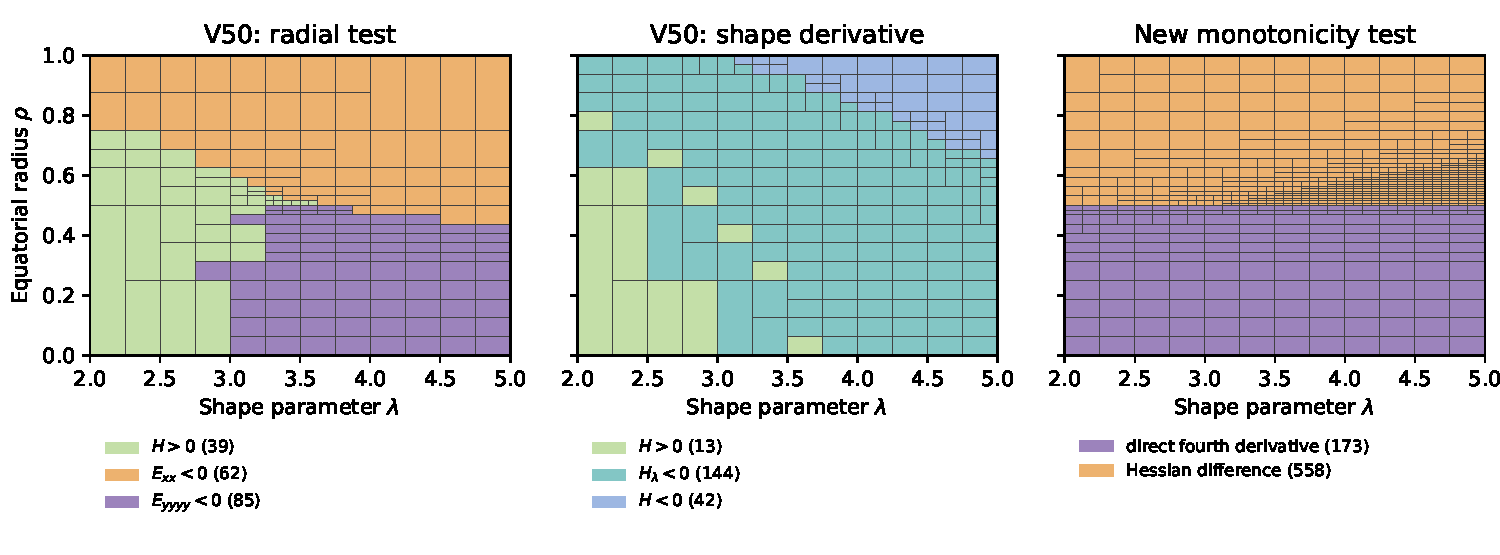
\includegraphics[width=\linewidth]{figures/gate_map.pdf}
\caption{完全に分割された三つの赤道上の検査における実際の終端長方形であり、凡例の数は終端の箱の個数である。最初の二つのパネルは、元の動径方向および形状方向の分割を再現する。三つ目は、ただ一つの符号についての新しい検査である。そこでの色の違いは、同じ四階導関数の二つの表示式を表す。}\label{fig:gate-map}
\end{figure}

\paragraph{記録された区間計算の結果。}
$[2,5]$上の幅$1/4$の十二個の形状スラブから出発した。新しい表には、直接の四階導関数の表示式に対する173個の終端の箱と、Hessianの差に対する558個の終端の箱が含まれる。半径の上端が$s$で半径の下端が正である外側の箱に対して、$H$の区間下界を$a$、$E_{xx}$の上界を$d$とする。$d<a$のとき、有理数$3(d-a)/s^2$は、その箱全体で$E_{yyyy}$の上界である。両方の種類の葉にわたる有理数の上端の最大値は次のとおりであった：
\[
             -109964349/2^{36} < -0.0016 .
\]
整数検査プログラムは、元の葉が出発時の各スラブを被覆することを検証する。第二の実装は、内側の箱では固定曲面エネルギーのTaylor係数を、外側の箱では弦方向における二つのHessian成分の差を積分する。これは元の箱の端点とモードを読み込む。全731個の箱において、局所的な細分の後、1,043個の小片上の上端の最大値は$-1/512$を下回った。したがって、どちらの実装からも上に示した上界が従う。補足ノートは、係数の公式、演算、および両方の被覆検査を与える。同じ元の検査を$1\leq\lambda\leq2$に拡張すると、176個の終端の箱（直接137個、弦39個）が得られ、上界は$-95257877/2^{36}$である。第二の評価プログラムもこれら176個の長方形を被覆し、399個の小片で、上端の最大値は$-0.00031$を下回った。この帯については、二つの独立な上界から、C3で用いる狭義の符号が従う。したがってこの帯では、記録された包囲が成り立つならば、C3における正の境界トレースから、赤道全体で$H>0$であることが従う。

\paragraph{記録された包囲が成り立つ場合の帰結。}
各$2\le\lambda\le5$に対して、$h'=\rho E_{yyyy}/3$であるから、関数$h(\rho)=H(\rho,0;\lambda)$は$(0,1)$上で狭義単調減少である。中心への連続性と、外側の端点における一階導関数のトレースへの連続性により、$h(0)>0>h(1)$ならば内部の半径がちょうど一つ得られ、そうでなければ一つも得られず、これは端点での値が零の場合も同様である。これが分類で用いる動径方向の一意性の議論である。縦方向の排除、二つの遷移の符号と位置、および半径の動きに対する$H_\lambda$は、別個の入力である。元の動径方向の実験には186個の葉があり、39個の箱が$H>0$を、62個が$E_{xx}<0$を、85個が$E_{yyyy}<0$を用いた。199個の葉からなる形状方向の被覆は、$H>0$、$H<0$、$H_\lambda<0$をそれぞれ13個、42個、144個の箱で用いた。これらの個数は実行時間のコストを比較するものではない。

図~\ref{fig:gate-map}において$\rho=1/2$のすぐ外側に箱が集中しているのは、表示の切り替えの位置で生じたものである。中心から離れた内部の重なりの上では、どちらの公式も利用できる。ここに示した計算は、$1/2$での固定した切断を用いる。


\subsection{境界と被覆の接続}
$1\le\lambda\le5$に対して、式~\eqref{eq:near_V}と式~\eqref{eq:window_V}の一様な正の下界は、$z\ne0$である境界点を排除する。境界の赤道上では動径方向成分のみが残る。その係数は$h_b$であり、これは$\bP$でのみ消える。次節の大きな扁長の場合の議論は、$\lambda\ge5$に対してすべての境界点を排除する。薄い扁平の場合の議論はC1--C2と$\lambda=1/32$を共有し、三つの扁長側の区間は端点$2$と$5$を共有する。命題~\ref{prop:sphere}と合わせて、これらの重なり合う範囲は、C1--C6から表~\ref{tab:classification}のすべての行を確立する。
